\chapter{Introduction}\label{ch:Introduction}
Electron tomography, often known as ET, is now the method of choice for determining the three-dimensional ultra-structure of organelles and cells at nanoscale resolutions. The 3D volume of the specimen can be reproduced by first collecting a tilted set of 2D transmission electron microscopy (TEM) images over a wide-angle range (usually $\pm$ 60\textdegree to 80\textdegree), and then computationally recombining the images. However, the low electron doses that are applicable to biological samples (which are typically less than 100 e\textsuperscript{-}/Å\textsuperscript{2}) result in extremely poor signal-to-noise ratios (SNR) in the tomograms that are produced as a result \cite{Frangakis2021}. The leading causes of the noise are the stochastic character of the events involving electron scattering and the constraints imposed by electron detection \cite{Joy2008}. In addition, flaws in the alignment of the tilt axis, beam-induced specimen deformation, and distortions that are inherent to electron lenses all contribute to the contamination of the TEM data \cite{Joy2008}. This leads to very tiny structural features, which are essential for interpreting the sophisticated cellular processes and chemical interactions, to get confused and distorted. Therefore, reducing the amount of noise in tomograms is one of the most crucial tasks in the preprocessing stage that comes before extracting data with biological significance.
\vspace{10pt}





Many alternative denoising methods have been used to enhance 3D ET reconstructions.
 To a certain extent, straightforward linear filters like median filtering, gaussian smoothing, and anisotropic diffusion filtration can reduce noise, but at the cost of a significant loss of high-resolution information \cite{Frangakis2001}. More enhanced regularization approaches such as total variation (TV) minimization and sparse coding exploit image priors to preserve edges and the rigidity of an image. However, these methods frequently require extensive parameter tuning to strike a balance between the removal of noise and the absorption of detailed information. Deep learning models such as \cite{Fernandez2023} have shown promise for 2D image denoising tasks. Unfortunately, 3D contextual information and the spatial relationships between coordinates cannot be successfully exploited by directly implementing such networks to slice-by-slice tomograms. Although several algorithms are capable of doing block-wise 3D denoising, they are restricted by computational restrictions \cite{Fernandez2023}. Other methods involve training on simulated data, which might not translate well to tomograms taken from actual data. 

\vspace{10pt}

While deep learning models like DnCNN \cite{Chen2017} have shown promise for 2D image denoising tasks, directly applying such networks to tomograms slice-by-slice fails to fully utilize 3D contextual information and spatial relationships between voxels. Some methods perform block-wise 3D denoising but are limited by computational constraints when scaling to large high-resolution volumes \cite{Xin2020}. Other techniques pretrain on simulated data which may not generalize well to real experimental tomograms with complex noise textures \cite{Xin2020}. Most existing deep learning approaches also lack interpretability into the learned features and struggle to denoise non-uniform noise distributions as encountered in practice.

\vspace{10pt}

More recently, neural radiance fields (NeRF) \cite{Mildenhall2020} have demonstrated unprecedented ability to synthesize photorealistic novel views of complex 3D scenes using a continuous volumetric representation. NeRFs learn a 5D radiance field where each 3D coordinate (X,Y,Z) is mapped to an emitted color (R,G,B) and volume density $\sigma$ using a standard multilayer perceptron (MLP). The key advantages of NeRF over other 3D deep learning representations are:

\begin{itemize}
\item  Coordinate-based MLPs better capture local spatial relationships compared to convolutional networks.
\item Continuous scene modeling enables synthesizing views from arbitrary poses.
\end{itemize}

In this work, we propose adapting NeRF for directly denoising 3D volumes reconstructed from tilt series electron tomography (ET) data. By training on pairs of noisy input and clean target volumes, the NeRF model may learn to infer superior denoised outputs closely matching the ground truth. The continuous volumetric modeling could outperform other 3D networks that lack such inductive bias. This approach could significantly enhance interpretability of structural details from electron tomograms.

\vspace{10pt}
However, directly applying NeRF for reconstructing volumes from noisy TEM tilt series poses significant challenges. The COLMAP structure-from-motion algorithm is utilized by the standard NeRF pipeline in order to perform camera pose estimation for each input image. The high noise levels of TEM projections, on the other hand, can make it difficult for COLMAP to properly establish the viewing angles. Because of this, it is challenging to train NeRF directly on raw TEM pictures that contain noise. Within the scope of this research, we suggest alterations to the NeRF framework that, if implemented, will make it possible to obtain a more accurate camera pose estimation from noisy TEM tilt series, where COLMAP fails to provide any camera poses. 

\vspace{10pt}

This study modifications to the NeRF framework to enable more robust camera pose estimation from noisy TEM tilt series. We also investigate training strategies and loss formulations to better condition the model on the noise characteristics of real ET data. This includes using robust loss functions that focus on structure rather than pixel intensities, as well as adaptive sampling and conditioning schemes. By adapting NeRF to handle noisy inputs in this manner, we aim to overcome the limitations of standard NeRF applied directly out-of-the-box to electron tomography volumes. Our noise-aware NeRF model could open new possibilities for high-fidelity 3D denoising and analysis of ET reconstructions.

\vspace{20pt}

\begin{figure}[thbp]
\centering
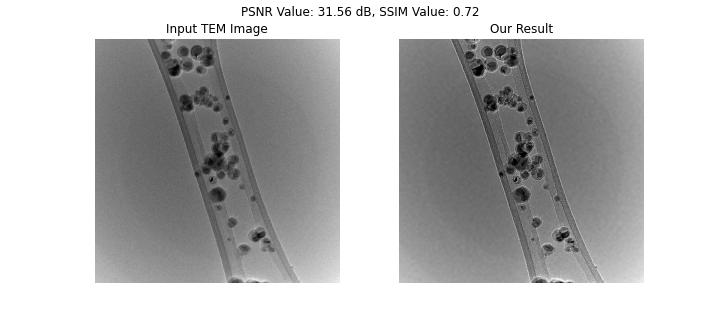
\includegraphics[width=1\textwidth]{img/comparison_image.jpg}
\caption{Comparative Analysis of Original TEM Images and Enhanced Outputs.}\label{fig: Comparative Analysis of Original TEM Images and Enhanced Outputs}
\end{figure}


A visual comparison between the original TEM images and the outcomes produced by our suggested method in Figure \ref{fig: Comparative Analysis of Original TEM Images and Enhanced Outputs}. This contrast draws attention to the difficulties caused by the noise in the original data and emphasizes how our method can improve image quality and lead to more precise analysis. Our innovative denoising technique was motivated by the significant reduction in noise and improvement in clarity, as illustrated in the picture. It demonstrates the significant influence that efficient noise reduction can have on TEM picture interpretability, which is necessary for precise 3D reconstruction and later biological investigation.

\vspace{10pt}